\subsection*{Changable Ring Oscillator}

\begin{figure}[H]
\centering
\tikzstyle{dot} = [draw,shape=circle,fill=black, scale =.3]
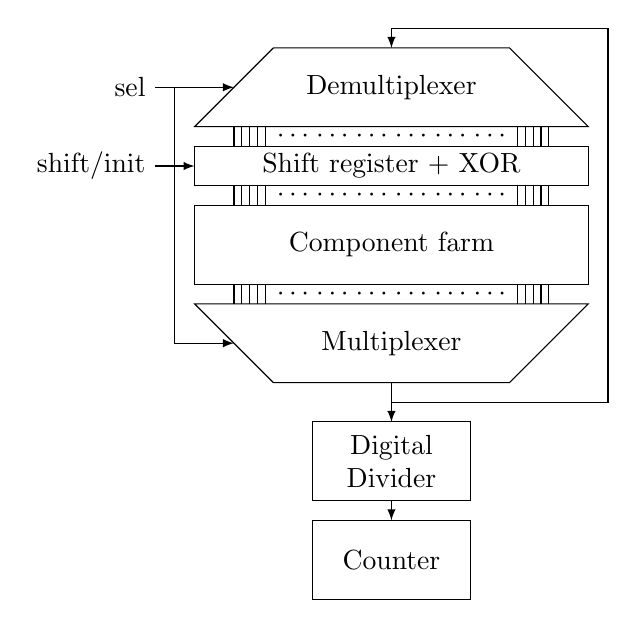
\begin{tikzpicture}
% Multiplexer and demultiplexer
\draw (1.5,6.5) -- (4.5,6.5) -- (5.5,5.5) -- (0.5,5.5) --  (1.5,6.5);
\node at (3,6) {Demultiplexer};
\draw (1.5,2.25) -- (4.5,2.25) -- (5.5,3.25) -- (0.5,3.25) --  (1.5,2.25);
\node at (3,2.75) {Multiplexer};

%components with connects
\draw  (0.5,5.25) rectangle (5.5,4.75) node[pos=.5]{Shift register + XOR};
\draw 
(1,4.5) -- (1,4.75)
(1.1,4.5) -- (1.1,4.75)
(1.2,4.5) -- (1.2,4.75)
(1.3,4.5) -- (1.3,4.75)
(1.4,4.5) -- (1.4,4.75);
\draw 
(4.6,4.5) -- (4.6,4.75)
(4.7,4.5) -- (4.7,4.75)
(4.8,4.5) -- (4.8,4.75)
(4.9,4.5) -- (4.9,4.75)
(5,4.5) -- (5,4.75);
\node at (1.75,4.625) {$\cdots$};
\node at (2.25,4.625) {$\cdots$};
\node at (2.75,4.625) {$\cdots$};
\node at (3.25,4.625) {$\cdots$};
\node at (3.75,4.625) {$\cdots$};
\node at (4.25,4.625) {$\cdots$};


\draw  (0.5,4.5) rectangle (5.5,3.5) node[pos=.5]{Component farm};
\draw 
(1,5.25) -- (1,5.5)
(1.1,5.25) -- (1.1,5.5)
(1.2,5.25) -- (1.2,5.5)
(1.3,5.25) -- (1.3,5.5)
(1.4,5.25) -- (1.4,5.5);
\draw 
(4.6,5.25) -- (4.6,5.5)
(4.7,5.25) -- (4.7,5.5)
(4.8,5.25) -- (4.8,5.5)
(4.9,5.25) -- (4.9,5.5)
(5,5.25) -- (5,5.5);
\node at (1.75,5.375) {$\cdots$};
\node at (2.25,5.375) {$\cdots$};
\node at (2.75,5.375) {$\cdots$};
\node at (3.25,5.375) {$\cdots$};
\node at (3.75,5.375) {$\cdots$};
\node at (4.25,5.375) {$\cdots$};
\draw 
(1,3.25) -- (1,3.5)
(1.1,3.25) -- (1.1,3.5)
(1.2,3.25) -- (1.2,3.5)
(1.3,3.25) -- (1.3,3.5)
(1.4,3.25) -- (1.4,3.5);
\draw 
(4.6,3.25) -- (4.6,3.5)
(4.7,3.25) -- (4.7,3.5)
(4.8,3.25) -- (4.8,3.5)
(4.9,3.25) -- (4.9,3.5)
(5,3.25) -- (5,3.5);
\node at (1.75,3.375) {$\cdots$};
\node at (2.25,3.375) {$\cdots$};
\node at (2.75,3.375) {$\cdots$};
\node at (3.25,3.375) {$\cdots$};
\node at (3.75,3.375) {$\cdots$};
\node at (4.25,3.375) {$\cdots$};

% feedback, counter and digital divider
\draw  (2,0.5) rectangle (4,-0.5) node[pos=.5, align=center]{Counter};
\draw [>=latex, ->](3,0.75) -- (3,0.5);
\draw  (2,1.75) rectangle (4,0.75) node[pos=.5, align=center]{Digital\\Divider};
\draw [>=latex, ->](3,2.25) -- (3,1.75);
\draw [>=latex, ->](3,2) -- (5.75,2) -- (5.75,6.75) -| (3,6.5);

%enable and select
\draw [>=latex, ->] (0.25,6) |- (1,2.75);
\draw [>=latex, ->] (0,6) -- (1,6);
\node [anchor=east] at (0,6) {sel};
\draw [>=latex, ->] (0,5) -- (0.5,5);
\node [anchor=east] at (0,5) {shift/init};
\end{tikzpicture}

\caption{Changable Ring Oscillator}
\label{tkz:changableRingOscillator}
\end{figure}

\begin{figure}[H]
\centering
\tikzstyle{dot} = [draw,shape=circle,fill=black, scale =.3]
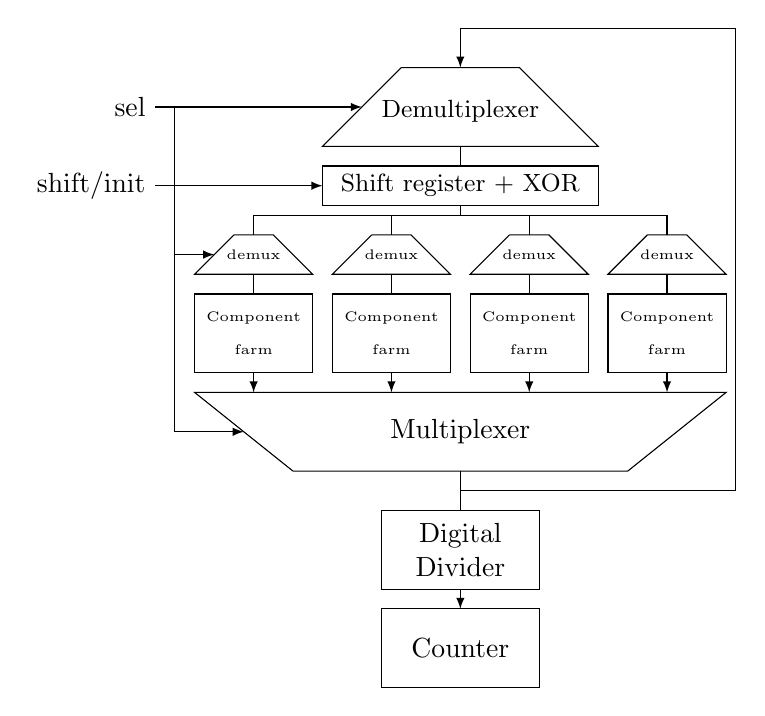
\begin{tikzpicture}
% Multiplexer and demultiplexer
\draw (2.625,8.25) -- (4.125,8.25) -- (5.125,7.25) -- (1.625,7.25) --  (2.625,8.25);
\node at (3.375,7.7) {\small{Demultiplexer}};
\draw (1.25,3.125) -- (5.5,3.125) -- (6.75,4.125) -- (0,4.125) --  (1.25,3.125);
\node at (3.375,3.625) {Multiplexer};

%shift register with connects
\draw  (1.625,7) rectangle (5.125,6.5) node[pos=.5]{\small{Shift register + XOR}};
\draw [>=latex, -](3.375,6.5) |- (0.75,6.375) -- (0.75,6.125);
\draw [>=latex, -](3.375,6.375) -| (6,6.125);
\draw [>=latex, -](4.25,6.375) -- (4.25,6.125);
\draw [>=latex, -](2.5,6.375) -- (2.5,6.125);

% component farm piece
\draw  (0,5.375) rectangle (1.5,4.375) node[pos=.5, align = center]{\tiny{Component}\\\tiny{farm}};
\draw (0.5,6.125) -- (1,6.125) -- (1.5,5.625) -- (0,5.625) --  (0.5,6.125);
\draw [>=latex, -] (0.75,5.625) -- (0.75,5.375);
\draw [>=latex, ->] (0.75,4.375) -- (0.75,4.125);
\node at (0.75,5.875) {\tiny{demux}};

% component farm piece
\draw  (1.75,5.375) rectangle (3.25,4.375) node[pos=.5, align = center]{\tiny{Component}\\\tiny{farm}};
\draw (2.25,6.125) -- (2.75,6.125) -- (3.25,5.625) -- (1.75,5.625) --  (2.25,6.125);
\draw [>=latex, -] (2.5,5.625) -- (2.5,5.375);
\draw [>=latex, ->] (2.5,4.375) -- (2.5,4.125);
\node at (2.5,5.875) {\tiny{demux}};

% component farm piece
\draw  (3.5,5.375) rectangle (5,4.375) node[pos=.5, align = center]{\tiny{Component}\\\tiny{farm}};
\draw (4,6.125) -- (4.5,6.125) -- (5,5.625) -- (3.5,5.625) --  (4,6.125);
\draw [>=latex, -] (4.25,5.625) -- (4.25,5.375);
\draw [>=latex, ->] (4.25,4.375) -- (4.25,4.125);
\node at (4.25,5.875) {\tiny{demux}};

% component farm piece
\draw  (5.25,5.375) rectangle (6.75,4.375) node[pos=.5, align = center]{\tiny{Component}\\\tiny{farm}};
\draw (5.75,6.125) -- (6.25,6.125) -- (6.75,5.625) -- (5.25,5.625) --  (5.75,6.125);
\draw [>=latex, -] (6,5.625) -- (6,5.375);
\draw [>=latex, ->] (6,4.375) -- (6,4.125);
\node at (6,5.875) {\tiny{demux}};

% feedback, counter and digital divider
\draw  (2.375,1.375) rectangle (4.375,0.375) node[pos=.5, align=center]{Counter};
\draw [>=latex, ->](3.375,1.625) -- (3.375,1.375);
\draw  (2.375,2.625) rectangle (4.375,1.625) node[pos=.5, align=center]{Digital\\Divider};
\draw [>=latex, -](3.375,3.125) -- (3.375,2.625);
\draw [>=latex, ->](3.375,2.875) -- (6.875,2.875) -- (6.875,8.75) -| (3.375,8.25);

%enable and select
\draw [>=latex, ->] (-0.25,7.75) |- (0.625,3.625);
\draw [>=latex, ->] (-0.5,7.75) -- (2.125,7.75);
\node [anchor=east] at (-0.5,7.75) {sel};
\draw [>=latex, ->] (-0.5,6.75) -- (1.625,6.75);
\node [anchor=east] at (-0.5,6.75) {shift/init};

\draw[>=latex, -] (3.375,7.25) -- (3.375,7);
\draw[>=latex, ->] (-0.25,5.875) -- (0.25,5.875);

\end{tikzpicture}

\caption{Changable Ring Oscillator 2}
\label{tkz:changableRingOscillator2}
\end{figure}



\begin{figure}[H]
\centering
\tikzstyle{dot} = [draw,shape=circle,fill=black, scale =.3]
\begin{tikzpicture}
% Buffer
\draw (3,2.75) node [buffer, scale=.6, rotate = -90] (buf1) at (3,3) {};

% DEMUX
\draw (3,2.75) node [and port, scale=.7, rotate = -90] (and1) at (3,1.5) {};
\draw
(buf1.out) -- (3,2.3)
(1.75,2.52) -| (and1.in 1)
(1.75,2.48) -| (and1.in 2);
\node [anchor=east] at (1.75,2.5) {sel};

% Shift register + XOR
\draw (3,2.75) node [xor port, scale=.7, rotate = -90] (xor1) at (3,0.25) {};
\draw  (3.75,2.25) rectangle (4.75,1.5) node[pos=.5]{SFF};
\draw 
(and1.out) -| (xor1.in 2)
(4.25,1.5) |- (xor1.in 1)
;

% DEMUX
\draw (3,2.75) node [and port, scale=.7, rotate = -90] (and2) at (3,-1) {};
\draw
(xor1.out) -- (3,-0.2)
(1.75,0.02) -| (and2.in 1)
(1.75,-0.02) -| (and2.in 2);
\node [anchor=east] at (1.75,0) {sel};

% actual component
\draw [fill=lightgray] (2,-1.25) rectangle (4,-2) node[pos=.5]{\small{component}};
\draw (and2.out) -- (3,-1.25);

% MUX
\draw (3,2.75) node [buffer, scale=.6, rotate = -90] (buf2) at (3,-2.5) {};
\draw (3,-2) -- (buf2.in);
\draw (3,2.75) node [and port, scale=.7, rotate = -90] (and3) at (3,-4) {};
\draw
(3,-3.19) -- (buf2.out)
(1.75,-2.98) -| (and3.in 1)
(1.75,-3.02) -| (and3.in 2);
\node [anchor=east] at (1.75,-3) {sel};

%loop
\draw (and3.out)-| (5,3.5) -| (buf1.in);
\end{tikzpicture}
\caption{critical path of dynamic ring oscillator}
\label{tkz:criticalPath}
\end{figure}